\chapter{Empirical Analysis}

This chapter should include
\begin{itemize}
  \item Execution environment
  \item Execution parameters
  \item Specific application profiles
  \item Result statistics (min/max/avg/stddev)
  \item Graphs with captions
  \item Practical (not theoretical) conclusions
\end{itemize}

\section{Execution environment}
The empirical analysis is based on the output of executing different
implementations on a machine with the following specifications:

%\begin{table}[!ht]
\begin{tabular}{|l|l|}
\hline
CPU & Intel\textregistered Core\texttrademark i5-2400 CPU @ 3.10GHz $\times$ 4
\\
\hline
Memory & Hynix/Hyundai 2048 MB DDR3 RAM @ 1333 MHz $\times$ 2 \\
\hline
\end{tabular}
%\end{table}

\section{Parameter value effects on performance}
\begin{figure}[!hbp]
    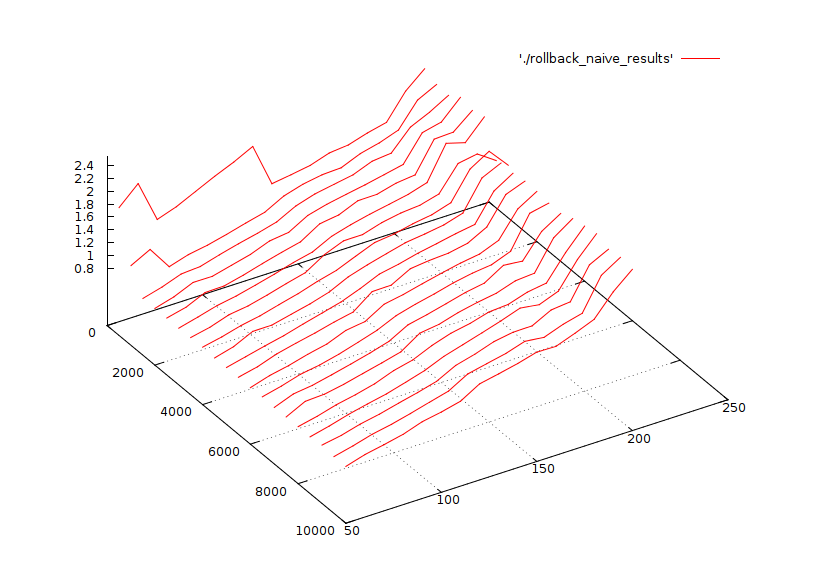
\includegraphics[width=\textwidth]{figures/rollback_naive_results_plot.png}
    \caption{Na\"ive rollback implementation: Plot of average time in ms per
    access operation for combinations of the two parameters: minimum distance
    between snapshots ranging from 50 to 250 and maximum allowed number of
    snapshots ranging from 1000 to 10000.}
    \label{fig:rollback_naive_results_plot.png}
\end{figure}

\begin{figure}[!hbp]
    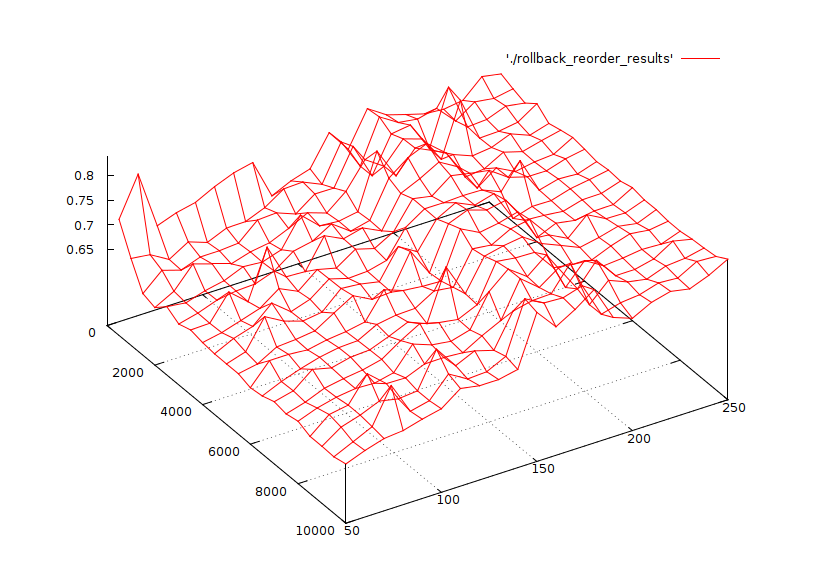
\includegraphics[width=\textwidth]{figures/rollback_reorder_results_plot.png}
    \caption{Rollback implementation with operations optimization: Plot of
    average time in ms per access operation for combinations of the two
    parameters: minimum distance between snapshots ranging from 50 to 250 and
    maximum allowed number of snapshots ranging from 1000 to 10000.}
    \label{fig:rollback_reorder_results_plot.png}
\end{figure}

\begin{figure}[!hbp]
    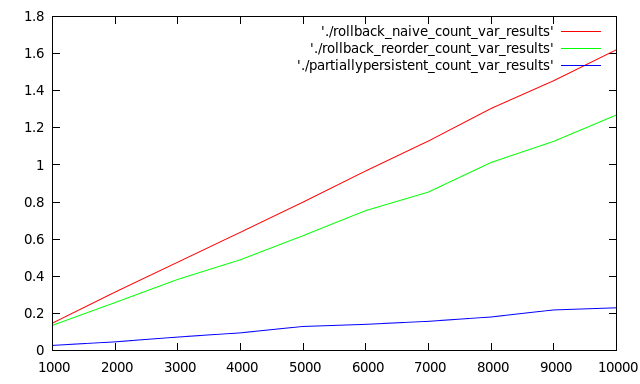
\includegraphics[width=\textwidth]{figures/rollback_results_count_var_plot.png}
    \caption{All implementations compared: When comparing all the
    implementations with the optimal parameters chosen for the rollback
    implementations, it is clear that the Node Copying method is far more
    efficient at accessing previous versions than either of the rollback
    implementations.}
    \label{fig:rollback_results_count_var_plot.png}
\end{figure}
